\newpage
\section{Objetivos}

Nessa pratica procuramos entender como funciona a rotação de um corpo, mais especificamente um com formato cilíndrico (roda de Maxwell), e a relação entre a sua dinâmica de rotação com o momento angular a fim de calculá-lo. Queremos provar que ela se conserva em todos os momentos do experimento, e também analisar o que acontece quando esse corpo sofre uma colisão plástica enquanto esta rodando.

Além disso, queremos estudar o fenômeno da precessão de corpos que giram, utilizando um giroscópio como objeto de estudo, para entender quais são os agentes que causam esse fato.

\begin{figure}[H]
  \centering
  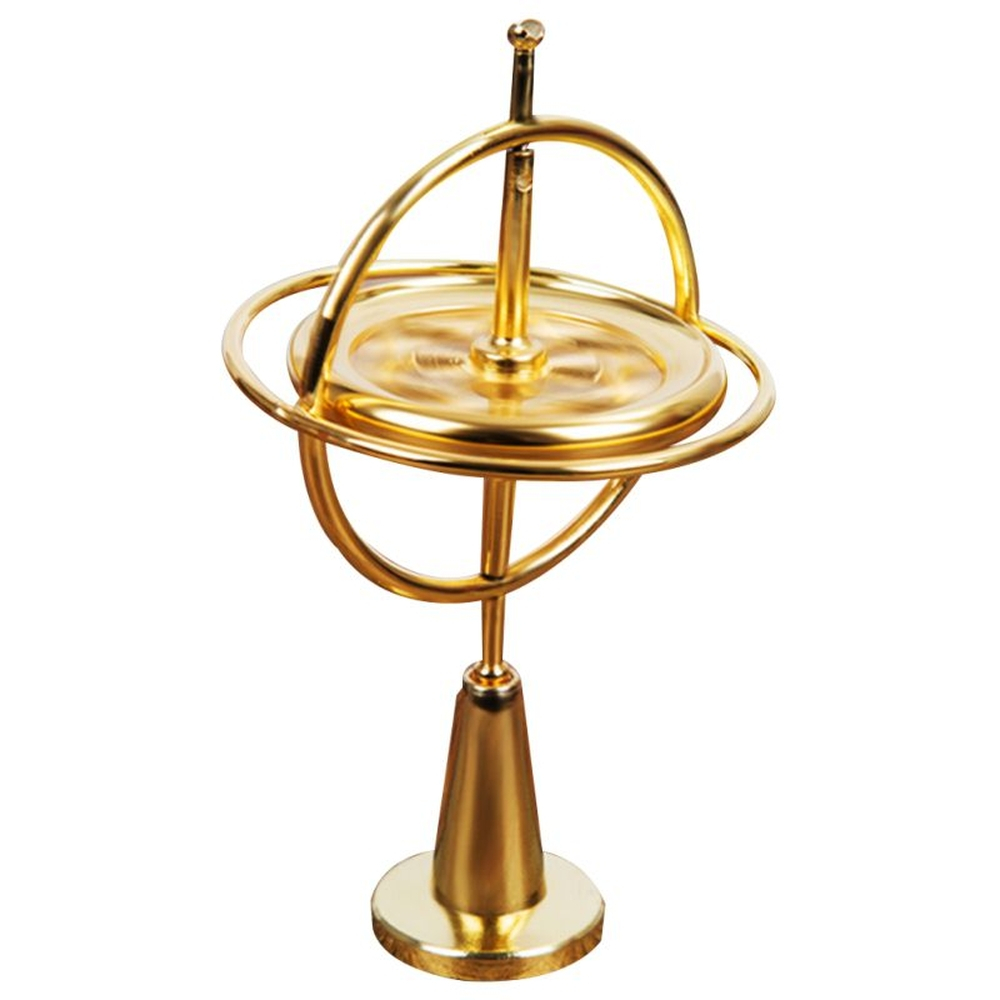
\includegraphics[scale=0.2]{images/giroscopio-brinquedo.jpg}
  \caption{Giroscópio}
\end{figure}
